\section{Durchführung}
\label{sec:Durchführung}
Der Aufbau des Versuches ist in folgender Abbildung schematisch dargestellt.
  \begin{figure}[H]
    \centering
      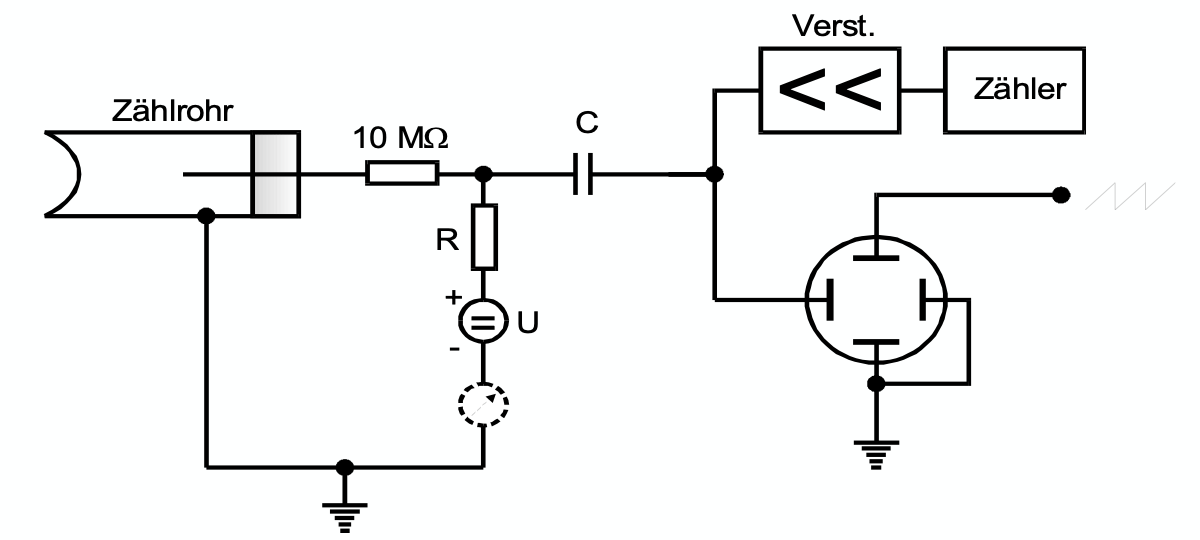
\includegraphics[scale=0.6]{content/AufbauV703.png}
<<<<<<< Updated upstream
      \caption{Der Versuchsaufbau, schematisch dargestellt. Quelle:\cite{AP01}}
||||||| constructed merge base
      \caption{Der Versuchsaufbau, schematisch dargestellt.}
=======
      \caption{Der Versuchsaufbau.}
>>>>>>> Stashed changes
      \label{fig:aufbau3}
  \end{figure}
<<<<<<< Updated upstream
||||||| constructed merge base

\label{sec:Durchführung}
=======
  Die Ladung $Q$, die auf dem Zähldraht innerhalb des Zählrohres aufgenommen wird, fließt über den
  Widerstand $R$. Dabei entsteht eine Spannung, die mit dem Kondensator ausgekoppelt und dann mithilfe
  des Verstärkers vergößert wird. Die vergößerte Spannung wird dann mit dem Oszillographen sichtbar
  gemacht. In Schritten von $\increment U = 10 \si{\volt}$ wurde die Anzahl Zerfälle innerhalb eines
  Zeitintervalls aufgenommen. Um sicherzustellen, dass    
\label{sec:Durchführung}
>>>>>>> Stashed changes
